\chapter{Конструкторский раздел}

Разрабатываемая оптимизация метода сжатия страниц памяти с использованием подсчета информационной энтропии состоит из следующих этапов:

\begin{enumerate}
	\item Вычисление значения информационной энтропии с помощью метода подсчета.
	\item Сравнение вычисленного значения информационной энтропии с пороговым значением.
	\item Сжатие страницы в случае, если полученное значение информационной энтропии меньше порогового значения.
\end{enumerate}

IDEF0-диаграмма первого уровня, формализующая основные этапы оптимизации сжатия страниц оперативной памяти, приведена на рисунке \ref{img:first-level}.
    
\includeimage
    {first-level}
    {f}
    {h}
    {1.0\textwidth}
    {IDEF0-диаграмма первого уровня}

\section{Схемы алгоритмов}

На рисунке \ref{img:get-sw-entropy} представлена схема алгоритма подсчета информационной энтропии методом скользящего окна.

\begin{figure}[H]
	\begin{center}
		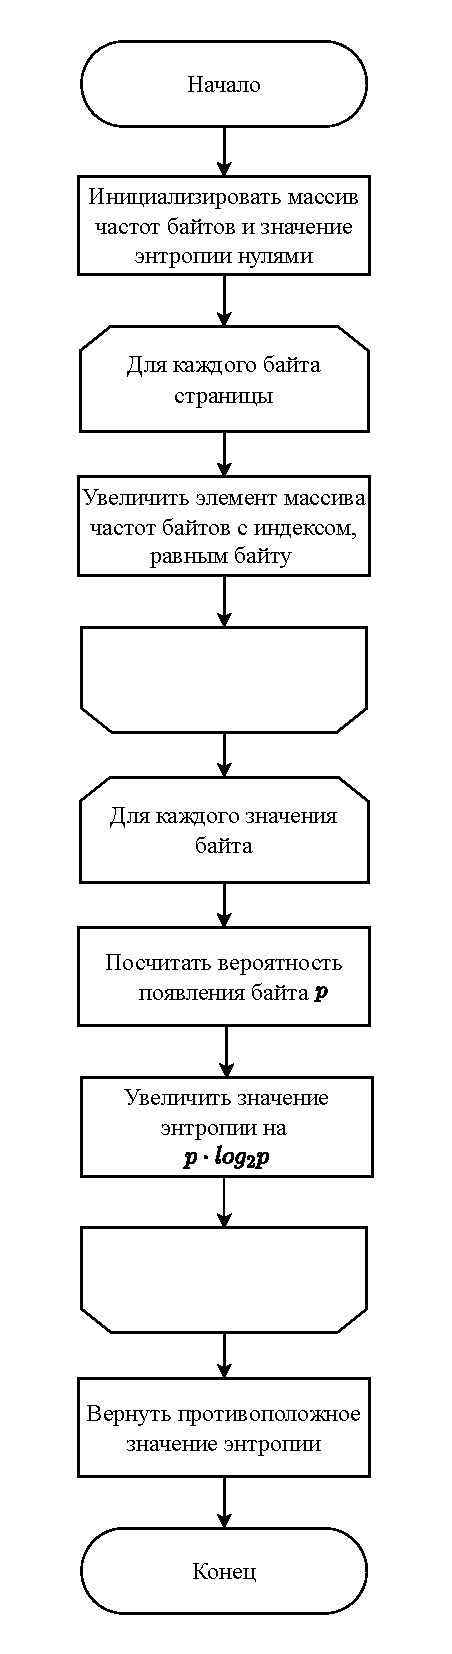
\includegraphics[scale=0.85]{inc/img/get-sw-entropy.pdf}
	\end{center}
	\captionsetup{justification=centering}
	\caption{Схема алгоритма метода скользящего окна}
	\label{img:get-sw-entropy}
\end{figure}

На рисунке  показана схема алгоритма подсчета информационной энтропии биномиальным методом.

На рисунке  приведена схема алгоритма сжатия страницы.

\section{Выбор структур данных}

\section{Структура программного обеспечения}

\section*{Вывод}

% Разработать основные этапы оптимизации метода сжатия страниц памяти с использованием подсчета информационной энтропии.
% Сформулировать и описать ключевые шаги метода подсчета информационной энтропии в виде схем алгоритмов. 
% Обосновать выбор структур данных.
% Описать взаимодействие компонентов системы.
